\chapter{LITERATURE REVIEW}
\label{chap-two}
Bridges are designed based on discrete events assuming that the initial material and structure properties remain constant through the life of the bridge. The purpose of the research described is to study condition dependent performance based design that considers the material and geometric properties as the structure ages, as well as the effects of multiple and discrete events on the achievement of prescribed limit states.

In this chapter, the current knowledge on aging of structures, damage indexes, corrosion and multiple earthquake loading is presented. Then the study gap is identified and the objectives of this research are defined.

\section{Corrosion}

One of the main phenomena that affect the long term behavior of RC structures is corrosion of the reinforcing steel.The main source of corrosion in RC structures is \textbf{chloride attack},thefore it is the one considered in this study.

The corrosion process of reinforced concrete structures under chloride attack consists in the loss of the protective film on the reinforcing steel surface, this process is known as \textbf{depassivation}, after which the initiation of corrosion occurs, the electrical resistivity and the oxygen content control corrosion. Figure \ref{fig:corr1} schematically show this process:

\begin{figure}[htbp]
\centering
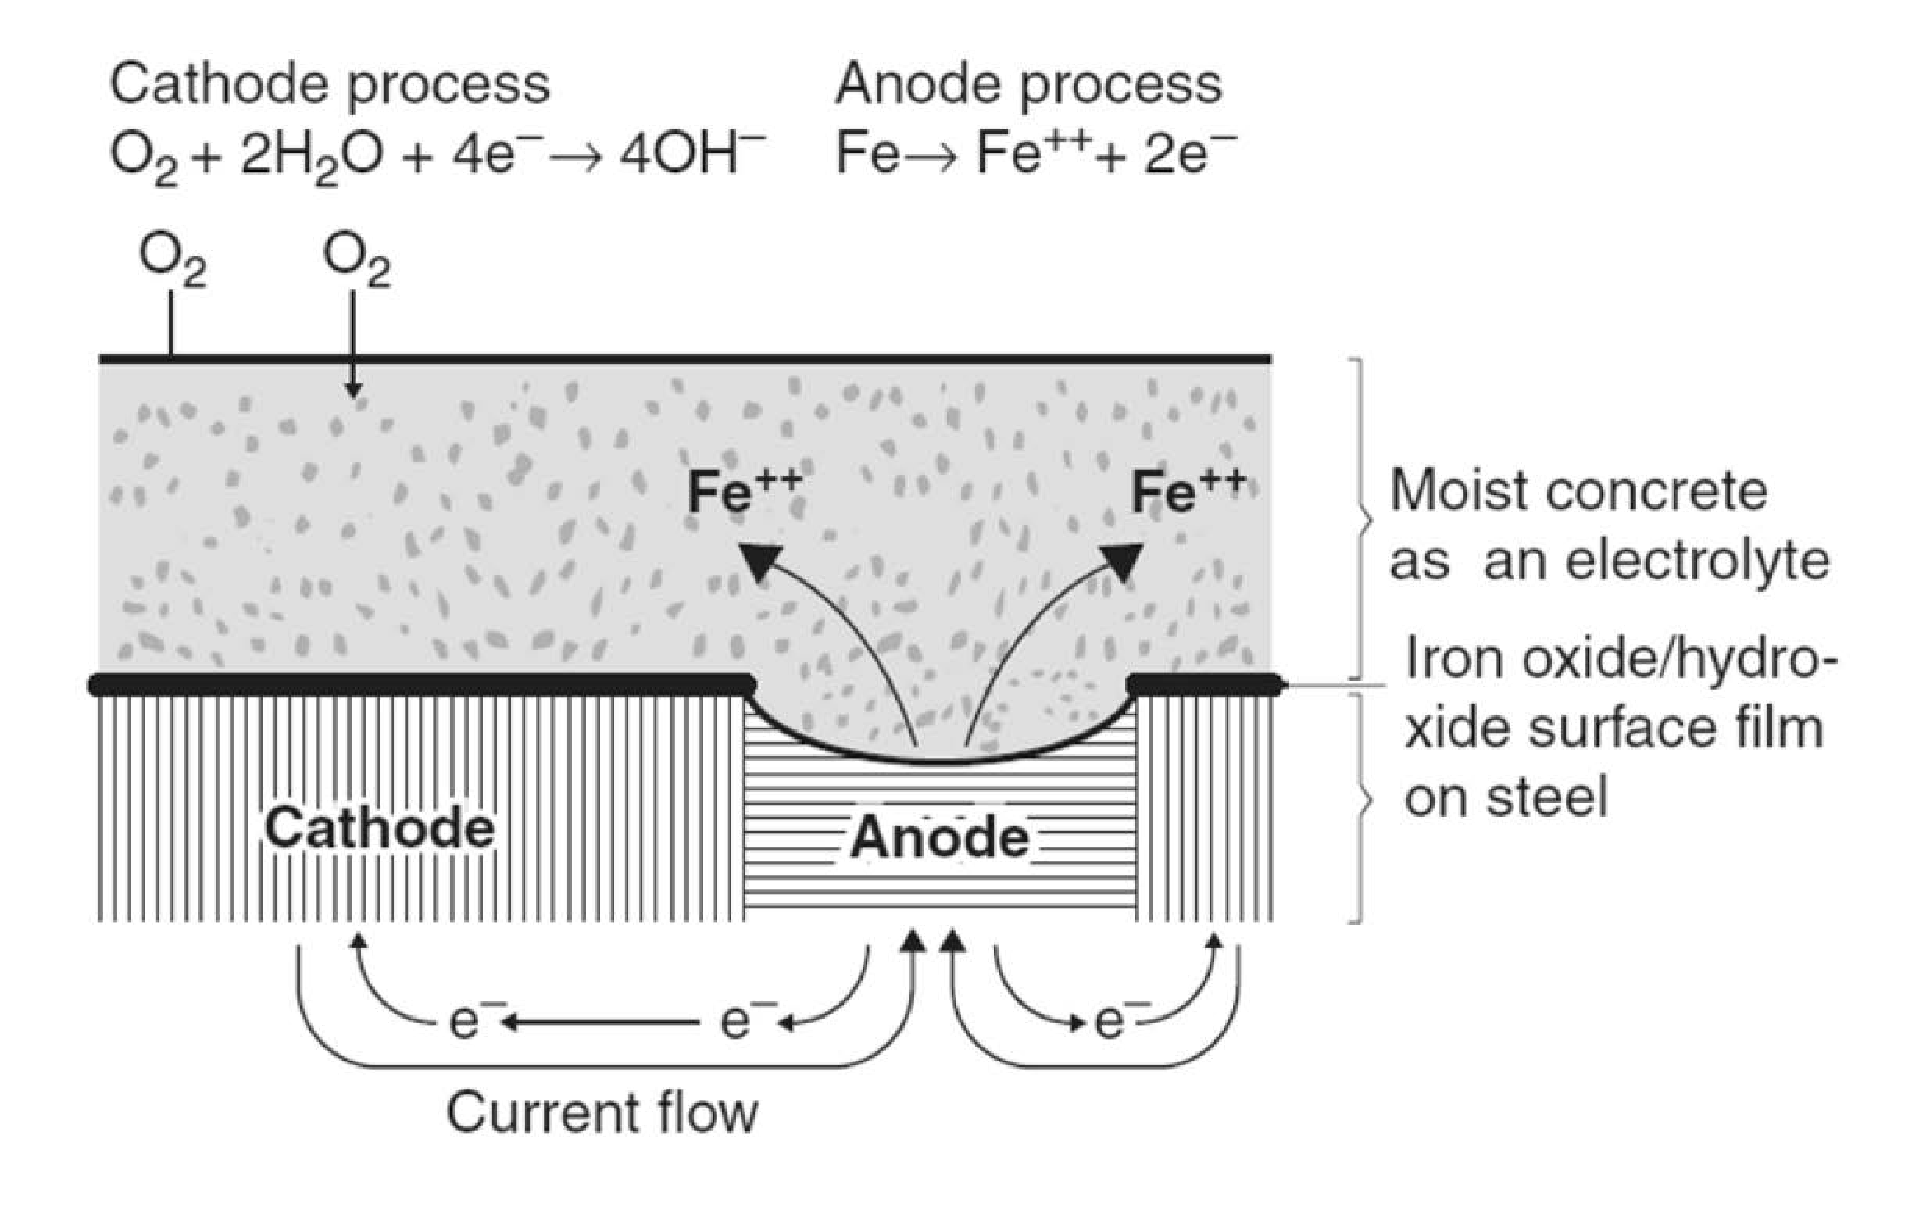
\includegraphics[width=0.9\textwidth]{Chapter-2/figs/Corrosion_Process}
\caption{Corrosion process in reinforcing steel bar \cite{Mehta2014}}
\label{fig:corr1}
\end{figure}

Corrosion plays an important role in the further deterioration of the seismic response of a structure. The parameters than describe corrosion are (1) Time to initiation of corrosion (Tcorr), (2) Corrosion growth in reinforcing steel, and (3) the mechanical properties of corroded reinforcing steel

\subsection{Time to corrosion}

 Researchers have  defined the corrosion initiation time as the time it takes to destroy the passive film of the reinforcing steel is destroyed and reinforcement starts corroding actively \cite{Thoft-Christensen}\cite{Stewart1998}\cite{Y.Liu1998a}. Fick's law was used to model the rate of chloride penetration into concrete as a function of concrete cover and time. Equation \eqref{eq:ficks_law} is solved in terms of the chloride ion concentration ($C(x,t)$), distance from concrete surface ($x$), time in seconds of exposure to chloride ions ($t$), and the chloride diffusion coefficient ($D_c$). The solution of equation \eqref{eq:ficks_law} resulted in equation \eqref{eq:two}.

\begin{equation}
	\frac{\partial C(x,t)}{\partial t} = D_c \frac{\partial C(x,t)}{\partial x^2}
	\label{eq:ficks_law}
\end{equation}
\newline

%\begin{equation}
  %C_(x,t)=c_{0} %\left[1-erf^{-1}\left(\frac{x}{2\sqrt[2]{D_c %t}}\right)\right]
%  \label{eq:two}
%\end{equation} 

%Equation \eref{eq:two}, was solved for t considering aa critical chloride corrosion threshold $C_r$ , and a equilibrium chloride concentration $C_0$, resulting in equation \eqref{eq.three} to calculate the time to corrosion ($T_{corr}$) in terms of \cite{Ghosh2010}. 

\begin{equation}
  T_{corr}=\frac{x^2}{4 D_c} \left[erf^{-1} \left(\frac{C_0-C_{cr}}{C_0} \right) \right]^{-2}
  \label{eq.three}
\end{equation} 

Mean values for $C_0$ and $C_r$ have been previously defined for environments that are controlled by \textbf{dicing salts} \cite{Ghosh2010}\cite{Weyers1994}\cite{Enright1998}.

%\textbf{Life 365}
%\newline
%
%Is a software developed by a consortium of companies of the cementitious materials industries and academic institutions. This software relies on the studies summarized above, mainly using the Thoft-Christensen model, but as opposed to assuming dicing environments only, this software uses a database of chlorides concentration for different location in the USA and Canada, which gives more accurate results depending on the location and environment in which the structure is located..
%
%While this is a more robust model to obtain the initiation of corrosion since it considers the location and environment of the structure and it also has the ability to include other durability issues, it is difficult to implement in a batch run mode since the program is in a closed format.
%\newline
%
%\textbf{Liu \& Weyers Model}
%\newline
%
%This model tries to calculate the time to initiation of corrosion by calculating the amount of corroding products that are needed to fill the voids in the concrete cover that will eventually generate cracking in this area and therefore initiate the accelerated corrosion of the reinforcing steel this is characterized through the following set of equations:
%
%
%\begin{equation}
%  W_{crit}=\rho_{rust} \left[ \pi \left[ \frac{C f'_t}{E_{ef}} \left( \frac{a^2+b^2}{a^2-b^2}+\nu_c \right)+d_o \right] D+ \frac{W_{st}}{\rho_{st}} \right]
%  \label{eq.four}
%\end{equation} 
%
%\begin{equation}
%  T_{cr}=\frac{W_{crit}^2}{2k_p}
%  \label{eq.five}
%\end{equation} 
%
%\begin{equation}
%  k_p=0.098 (\frac{1}{\alpha})\pi Di_{corr}
%  \label{eq.six}
%\end{equation} 
%
%$W_{crit}$: Critical amount of corrosion needed to induce cracking.
%
%$W_{st}$: Mass of corroded steel.
%
%$\rho_{rust}$: Density of rust material.
%
%$\rho_{st}$: Density of steel.
%
%$f'_t$: Tensile strength of the concrete. 
%
%$E_{ef}$: Effective elastic modulus of concrete $E_{ef}=\frac{E_c}{1+\phi_{crit}}$ 
%
%$\phi_{crit}$ Creep coefficient of the concrete.
%
%$D$: Diameter of bar.
%
%$d_o$: Thickness of pore band around the steel/concrete interface.
%
%$\nu_c$: Poisson's ratio of concrete.
%
%$C$: Cover depth
%
%$a=\frac{D+2d_o}{2}$
%
%$b=C+\frac{D+2d_o}{2}$
%
%This model however is limited to corrosion on concrete slabs, since a series of experiments were developed to generate these equations, however, it is able predict the time to corrosion with great accuracy.

\subsection{Rate of corrosion}

Stewart et al developed a model to calculate the corrosion rate  \cite{Vu2000}\cite{Stewart1998}. The corrosion rate describes the loss of steel cross section due to corrosion.   Corrosion rate is a function of the water to cement ratio ($w/c$) and the cover depth ($d_c$) shown in equation \eref{eq.CorrosionRate}.

%This model implies that corrosion rate decreases with time. As corrosion accumulates around the reinforcing steel, the corrosion byproducts prevent the uncorroded steel to react with the environment.

\begin{equation}
  i_{corr}=\frac{37.5(1-w/c)}{d_c}
  \label{eq.CorrosionRate}
\end{equation} 

In \fref{fig:hist1} the behavior of this model for different values of $w/c$ ratios is shown. In general, for large values of cover depth the rate of corrosion decreases rapidly and as the water cement ratio increases the rate of corrosion increases.
%
\begin{figure}[htbp]
\centering
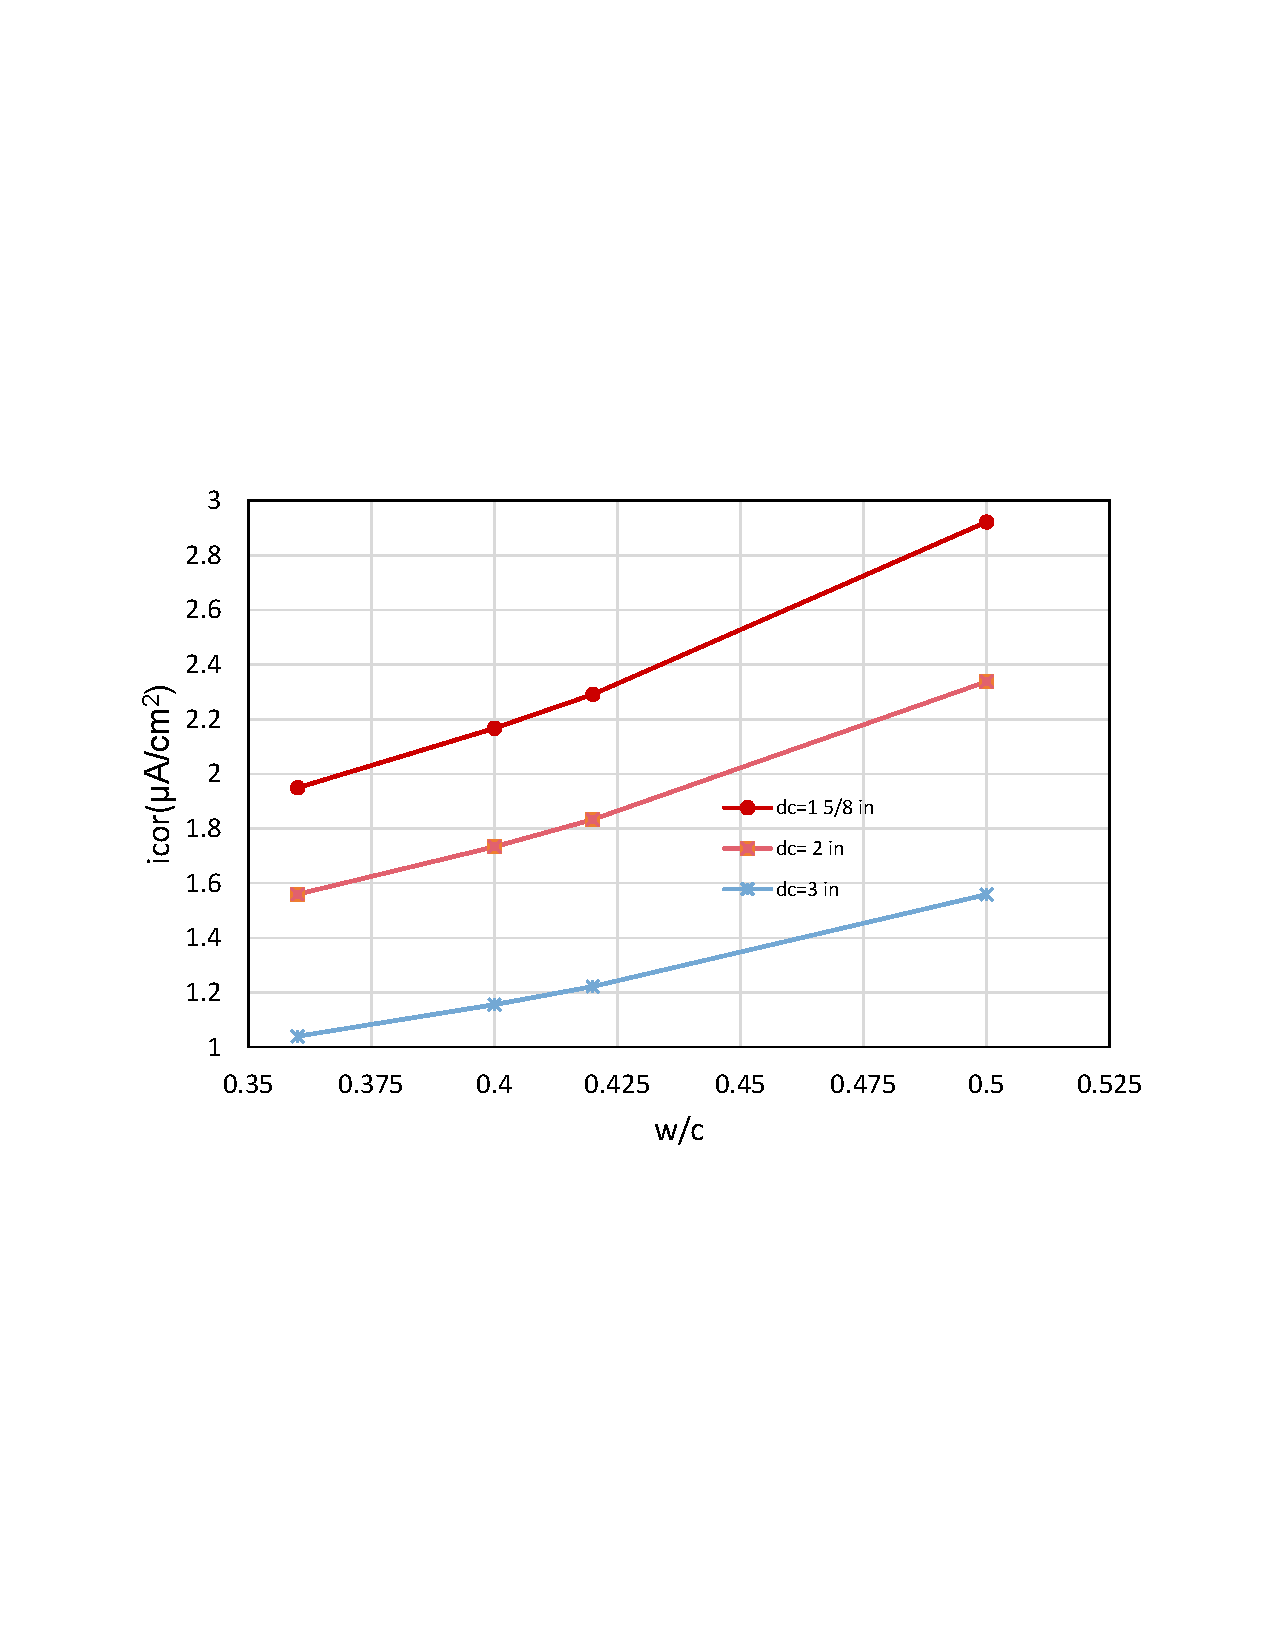
\includegraphics[width=0.85\textwidth]{Chapter-2/figs/wc_icor}
\caption{Concrete water to cement ratio vs rate of corrosion}
\label{fig:hist1}
\end{figure}

Vu et al proposed a model to describe the growth of corrosion as a function of the rate of corrosion clearly defined \cite{Vu2000}\cite{Stewart1998}\cite{Choe2008}\cite{Ghosh2010}. The proposed model is presented in equation \eref{eq.CorrosionEvolution}, this equation represents the reduction in diameter of reinforcing steel ($d_{corr}(t)$ as a function of time. For example consider a rebar with initial diameter ($d_{bi}$) of 3/4 inch diameter reinforcing steel with a concrete cover of 1-1/2” is using, and water to cement ratios ranging from 0.36-0.50, figure \fref{fig:DiameterEvolution} was developed.

\begin{equation}
  d_{corr}(t)=d_{bi}-\frac{1.0508(1-w/c)}{d_c} (t-t_{corr})^{0.71}
  \label{eq.CorrosionEvolution}
\end{equation} 

\begin{figure}[htbp]
\centering
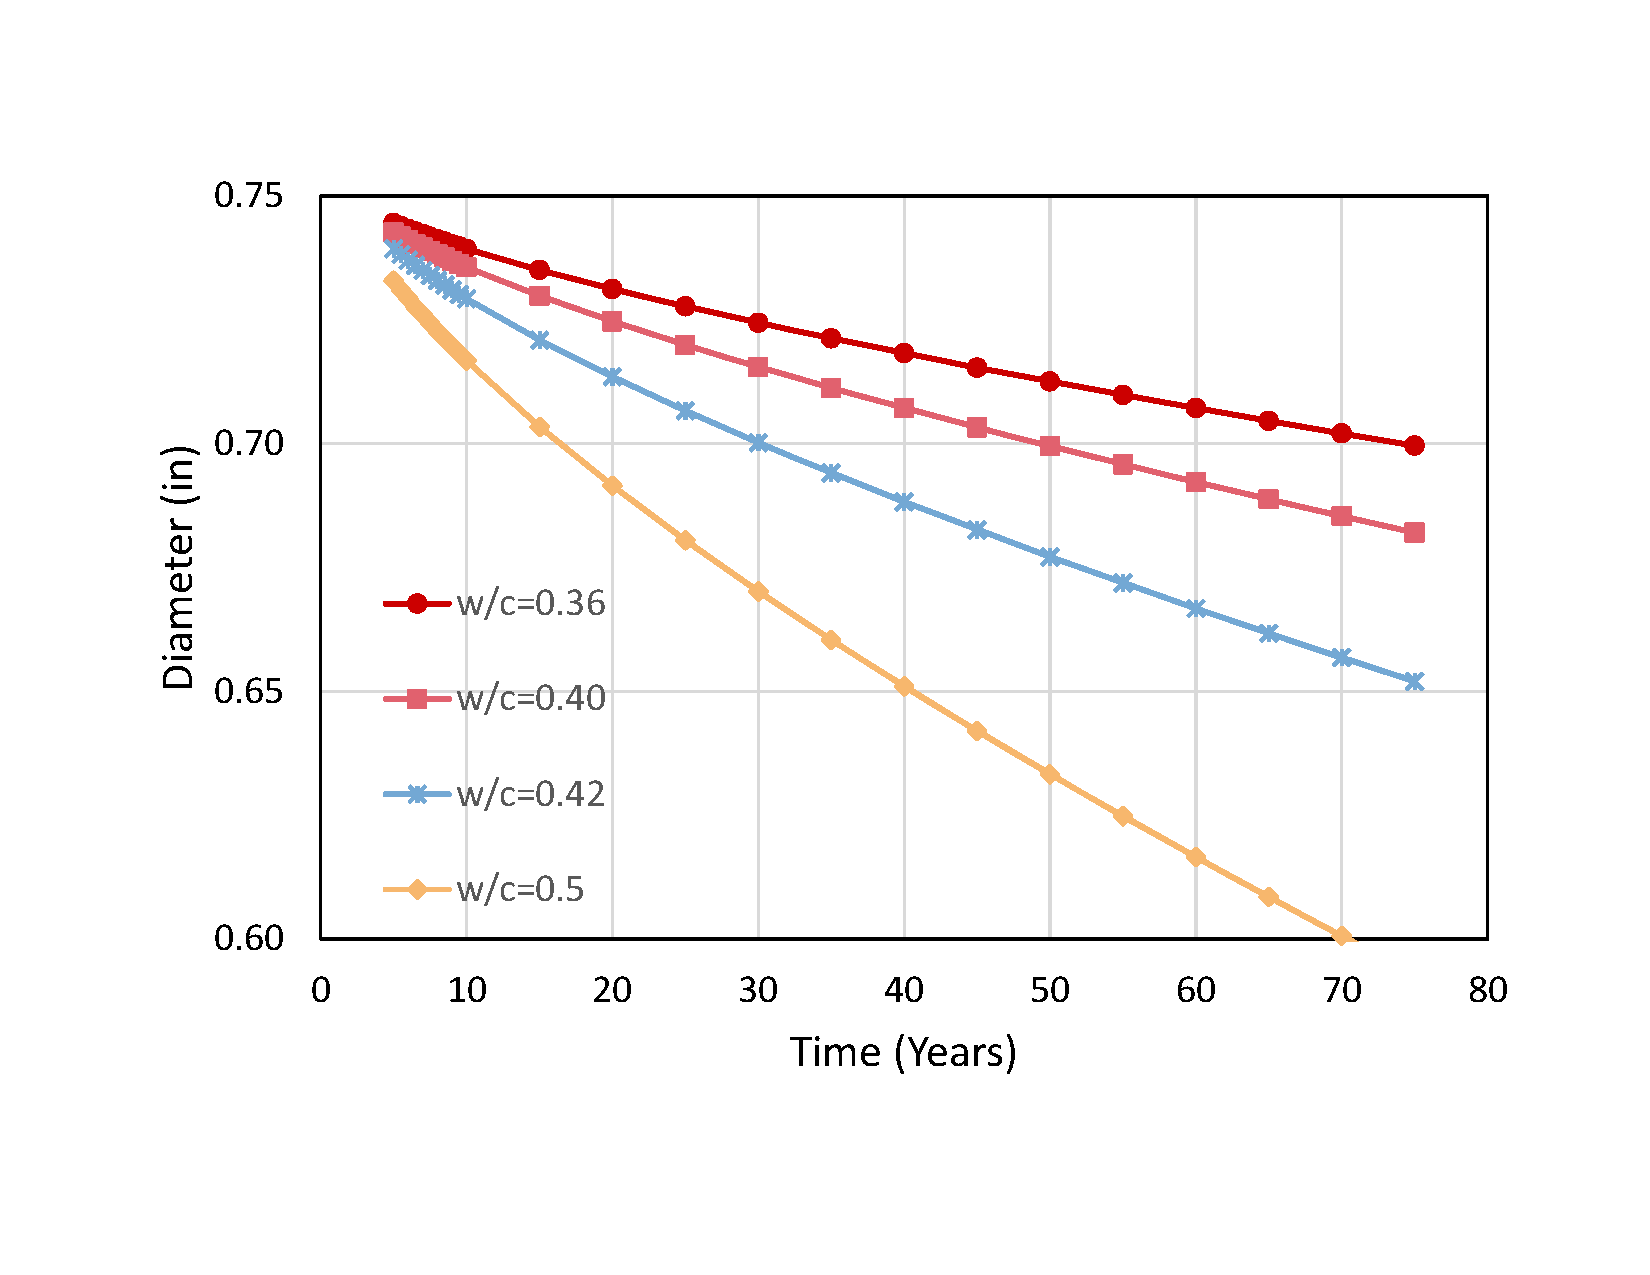
\includegraphics[width=0.85\textwidth]{Chapter-2/figs/DiameterDecrease}
\caption{Diameter decrease due to corrosion}
\label{fig:DiameterEvolution}
\end{figure}

The evolution of corrosion in reinforcing steel is expressed in the percent loss of mass of a rebar. Assuming uniform corrosion corrosion level is calculated as shown in equation \eref{eq.CorrosionLevel}.

\begin{equation}
	CL=\frac{d_{i}-d(t)}{d_{i}}*100%
  \label{eq.CorrosionLevel}
\end{equation} 

Using equation \eref{eq.CorrosionEvolution} with equation \eref{eq.CorrosionLevel}  the variation of corrosion level can be described as a fuction of time. Figure  \fref{fig:CorrosionLevel_Time} shows the results of this process.

\begin{figure}[htbp]
\centering
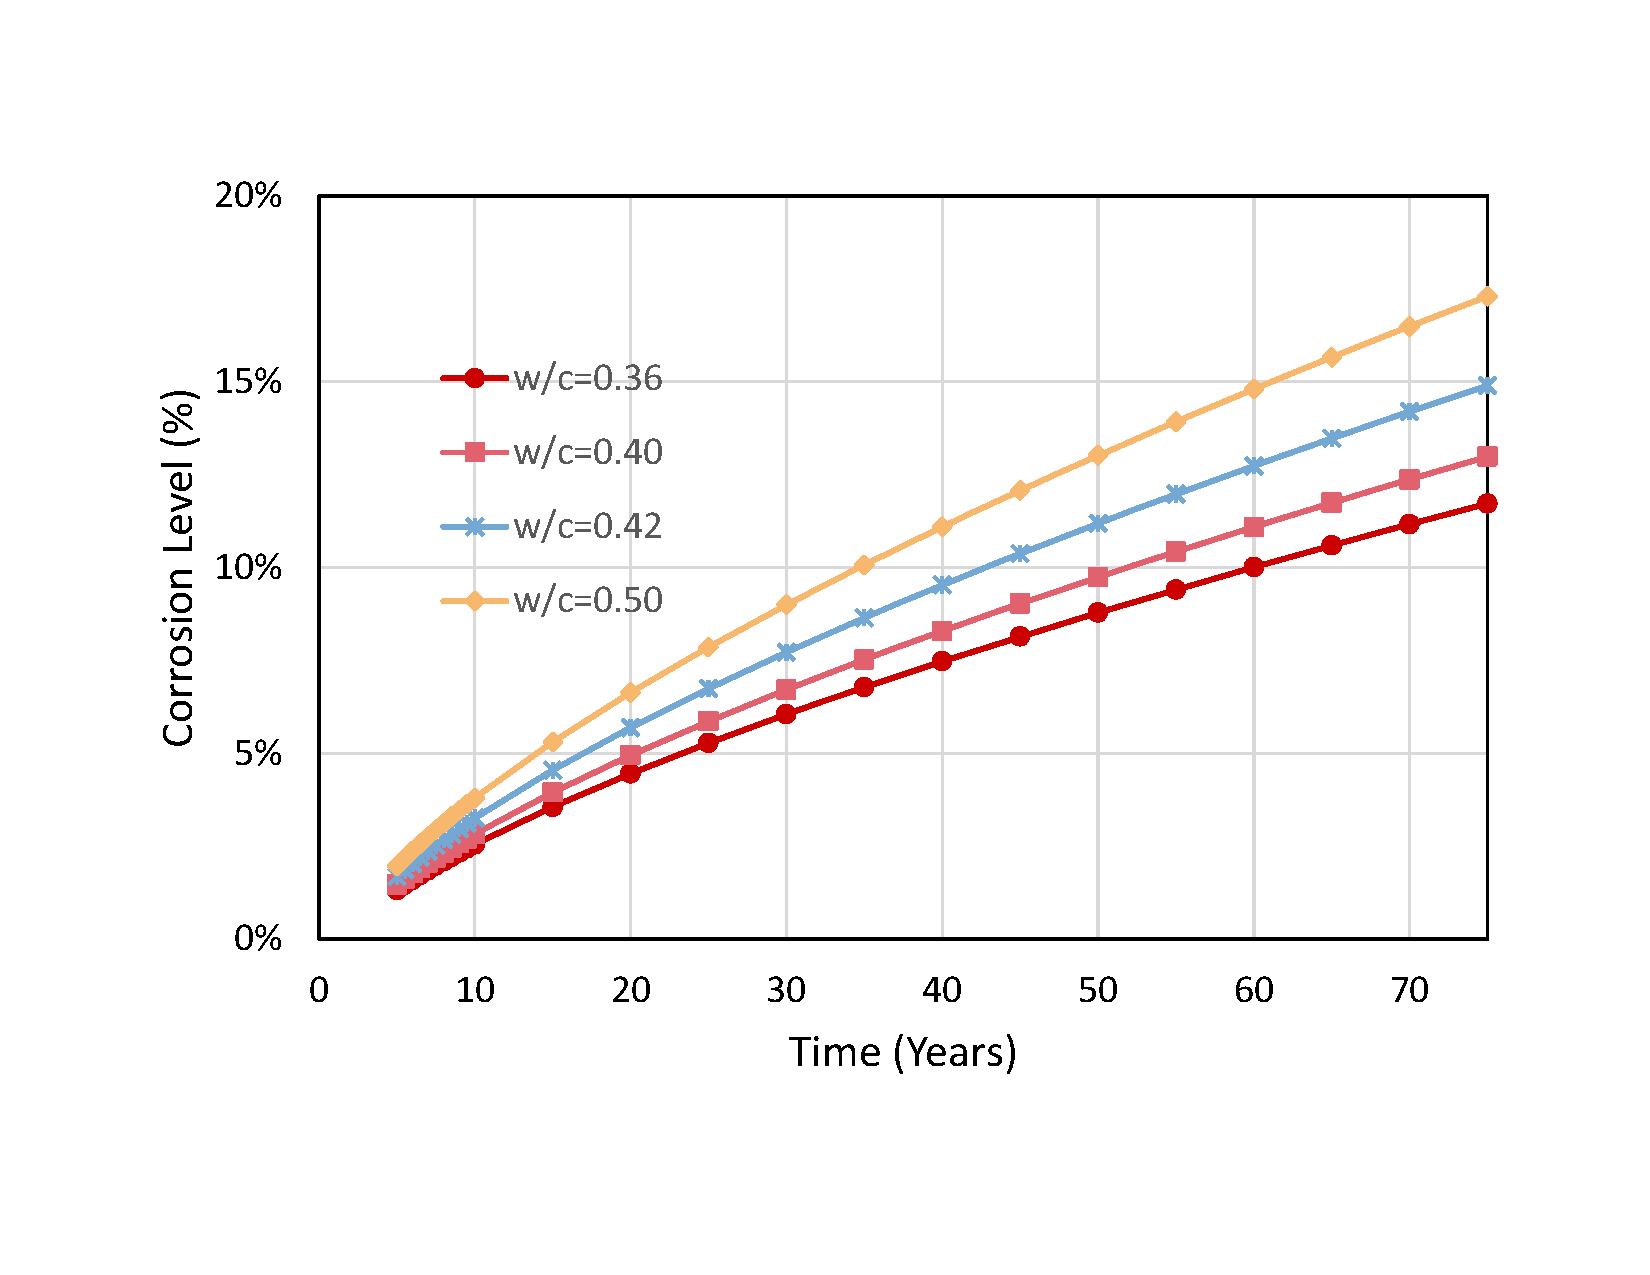
\includegraphics[width=0.85\textwidth]{Chapter-2/figs/CorrosionLevel}
\caption{Corrosion level vs time (years)}
\label{fig:CorrosionLevel_Time}
\end{figure}

\subsection{Corrosion modified properties of reinforcing steel bars}

Yuan et al \cite{Yuan2017a} performed experimental tests in corroded rebars and determined that the mechanical properties of steel change with the level of corrosion. The variation of the mechanical properties is shown in \eref{eq.eleven} for the yield strength and ultimate strength of the reinforcing steel.

\begin{equation}
  f_{y,C}=f_{yo}(1-0.021C)
  \label{eq.eleven}
\end{equation} 
\[
  f_{u,C}=f_{yo}(1.018-0.019C)
\]

\section{Steel strain aging}

\subsection{Metallurgical process}

It is generally accepted that strain aging is due to the diffusion of carbon and/or nitrogen atoms in solution to dislocations that have been generated by plastic deformation. Initially, an atmosphere of carbon and nitrogen atoms is formed along the length of a dislocation, immobilizing it. Extended aging, however, results in sufficient carbon and nitrogen atoms for precipitates to form along the length of the dislocation\cite{Overby2017}\cite{Hosseini2015}.

These precipitates impede the motion of subsequent dislocations and result in some hardening and loss in ductility. The extent of strain aging, which is a thermally activated process, depends primarily on aging time and temperature. In general, extended aging results in a saturation value above which further aging has no effect \cite{Restrepo-Posada1994}.

A second strengthening mechanism occurs when cold deformation (alone) is applied to steels. When dislocations break away for their pinning interstitial atoms and begin the movement causing slip they begin to intersect with each other. A complex series of interactions between the dislocations occurs, causing them to pin each other, decreasing their mobility. The decreased mobility also results in higher strength, lower ductility and lower toughness. As a result, cold deformed steels already have lowered ductility and toughness before any strain aging occurs and when heating follows cold deformation, the loss in ductility and toughness is greater. It is this combination of events that is the most damaging to the toughness of structural steels \cite{Momtahan2009}.

\subsection{Strain aging effects in structures}

Given the fact that that strain aging is the process by which steel after being subjected to large strains develops an increased strength and reduced ductility with time. It is  important to include it in a time dependent analysis. Furthermore strain aging will cause an increase in the strength of the plastic hinge and as a consequence plastic hinges may formed in regions of the structures that have not been designed for such demands. The effects of strain aging may also alter the transverse reinforcement due to cold bending, making them susceptible to brittle failure\cite{Momtahan2009}.

According to Restrepo-Posada\cite{Restrepo-Posada1994} most strain aging occurs in the first 37 days. Also \cite{Momtahan2009} studied strain aging effects with respect to time for different levels of pre-strains that ranged from $2\varepsilon_y - 10\varepsilon_y$ and for a time frame of 3 days to 50 days, from this study it was determined that a significant effect of strain aging took place from pre-strains $5\varepsilon_y$ and on. Strains higher than $15\varepsilon_y$ indicate a performance level in which substantial damage has been induced in the structure such that it is deemed unrepairable and therefore pre-strains higher that $15\varepsilon_y$ are unpractical and not studied by Momtahan et al\cite{Momtahan2009}.

Momtahan et al was able to correlate the increase in yield strength as a function of time and the pre-strain in reinforcing steel bars. The proposed equations are shown below:

\begin{figure}[htbp]
\centering
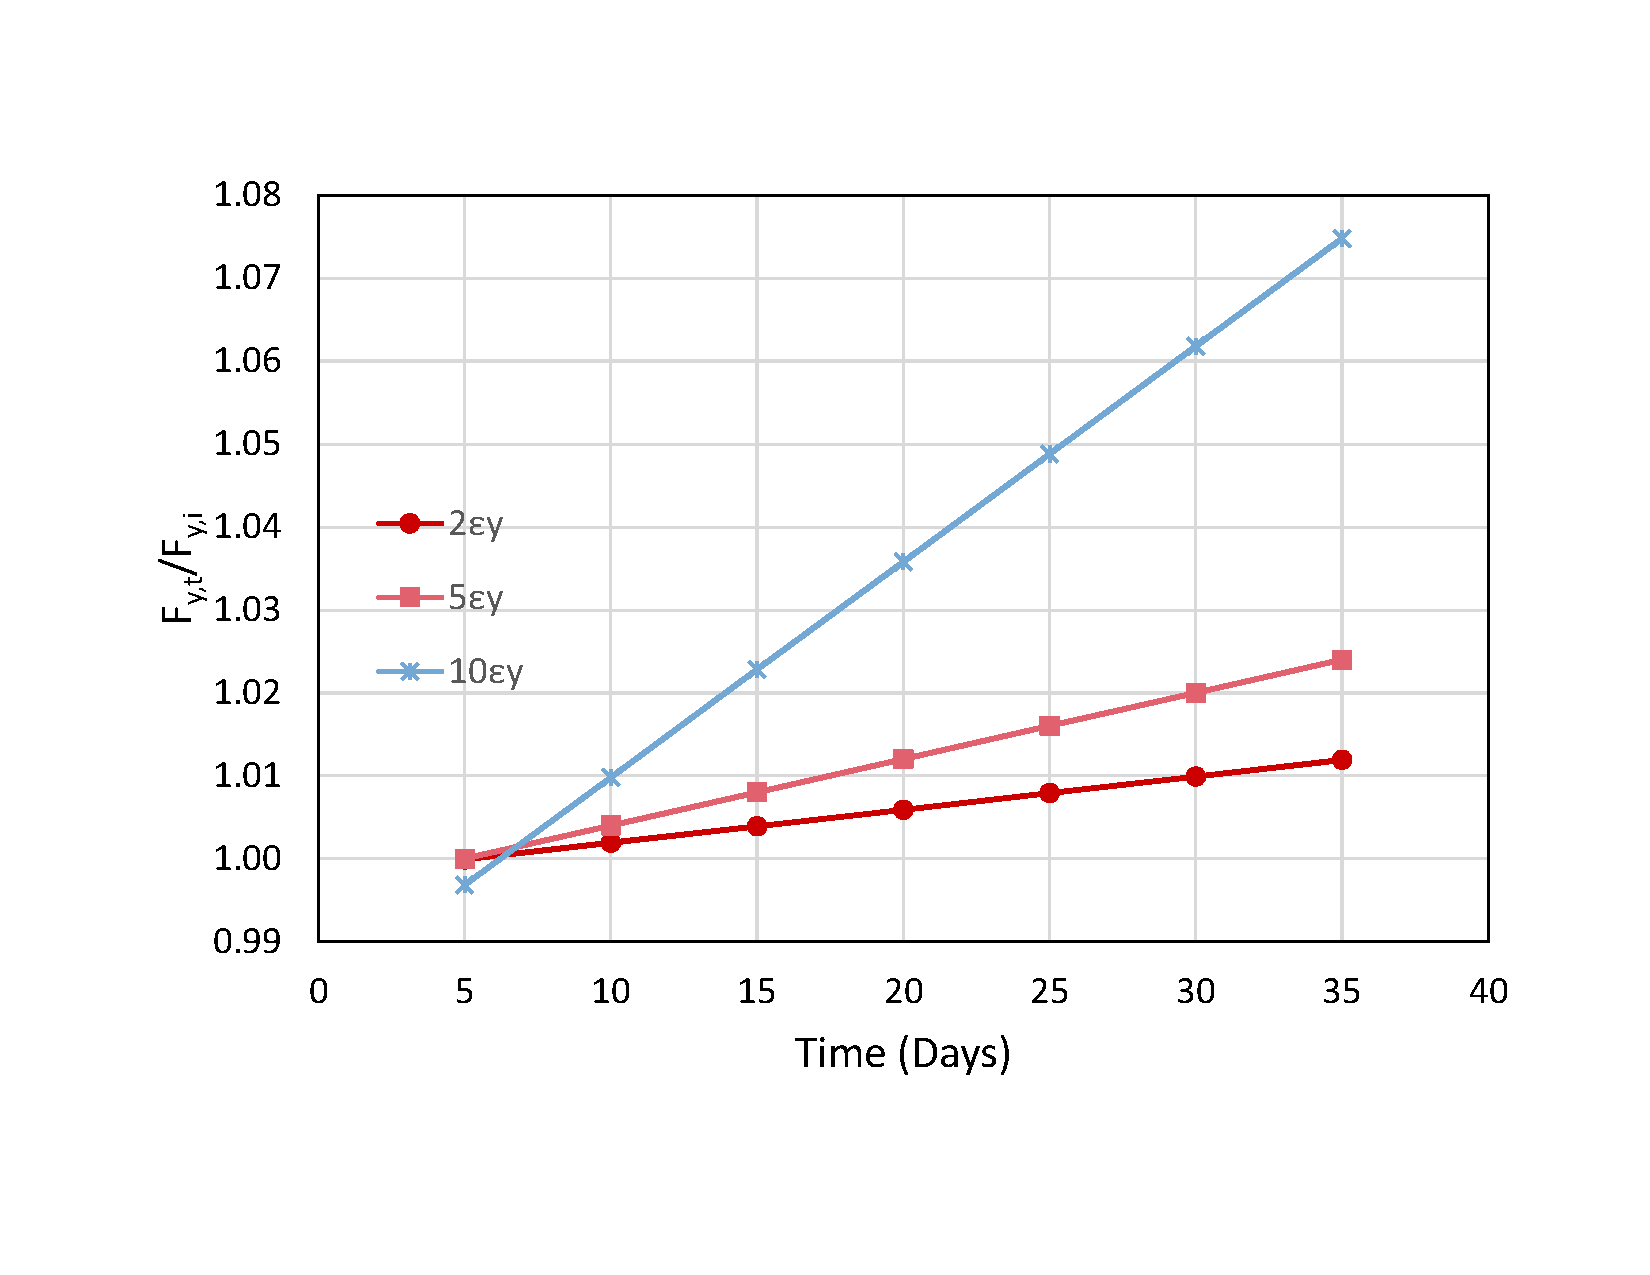
\includegraphics[width=0.7\textwidth]{Chapter-2/figs/StrainAging_TimeDependent}
\caption{Strain aging effect on yield strength vs time (days)}
\label{fig:hist4}
\end{figure}

For $10\varepsilon_y$

\begin{equation}
  \frac{f_y}{f_{yi}}=0.0026t+0.9838
  \label{eq.twelve}
\end{equation} 

For $5\varepsilon_y$

\begin{equation}
  \frac{f_y}{f_{yi}}=0.0008t+0.996
  \label{eq.thirteen}
\end{equation} 

For $2\varepsilon_y$

\begin{equation}
  \frac{f_y}{f_{yi}}=0.0004t+0.9979
  \label{eq.fourteen}
\end{equation} 

It is proposed to limit the increase in yield strength to the one obtained at 50 days which was the limit of scope of the study. These equations are plotted in \fref{fig:hist4}

\section{Damage Indexes}
The effect of cumulative damage in structures was studied by Park and Ang (1985) \cite{Young-JiPark1985} in their study the authors proposed the damage index as shown in Eq \ref{eq.DamageIndex}. The damage index was used as a measure to quantify damage in terms of the maximum experienced earthquake and the absorbed hysteretic energy.

\begin{equation}
  D=\frac{\Delta_{m}}{\Delta_{u}}-\beta \frac{E_h}{F_{y}\Delta{u}}
  \label{eq.DamageIndex}
\end{equation} 

$\Delta_{m}$: Maximum deformation under earthquake

$\Delta_{u}$: Ultimate deformation under monotonic loading

$F_{y}$: Calculated yield strength

$E_{h}$: Total hysteretic energy

$\beta$: Dimensionless constant 

\begin{figure}[htbp]
\centering
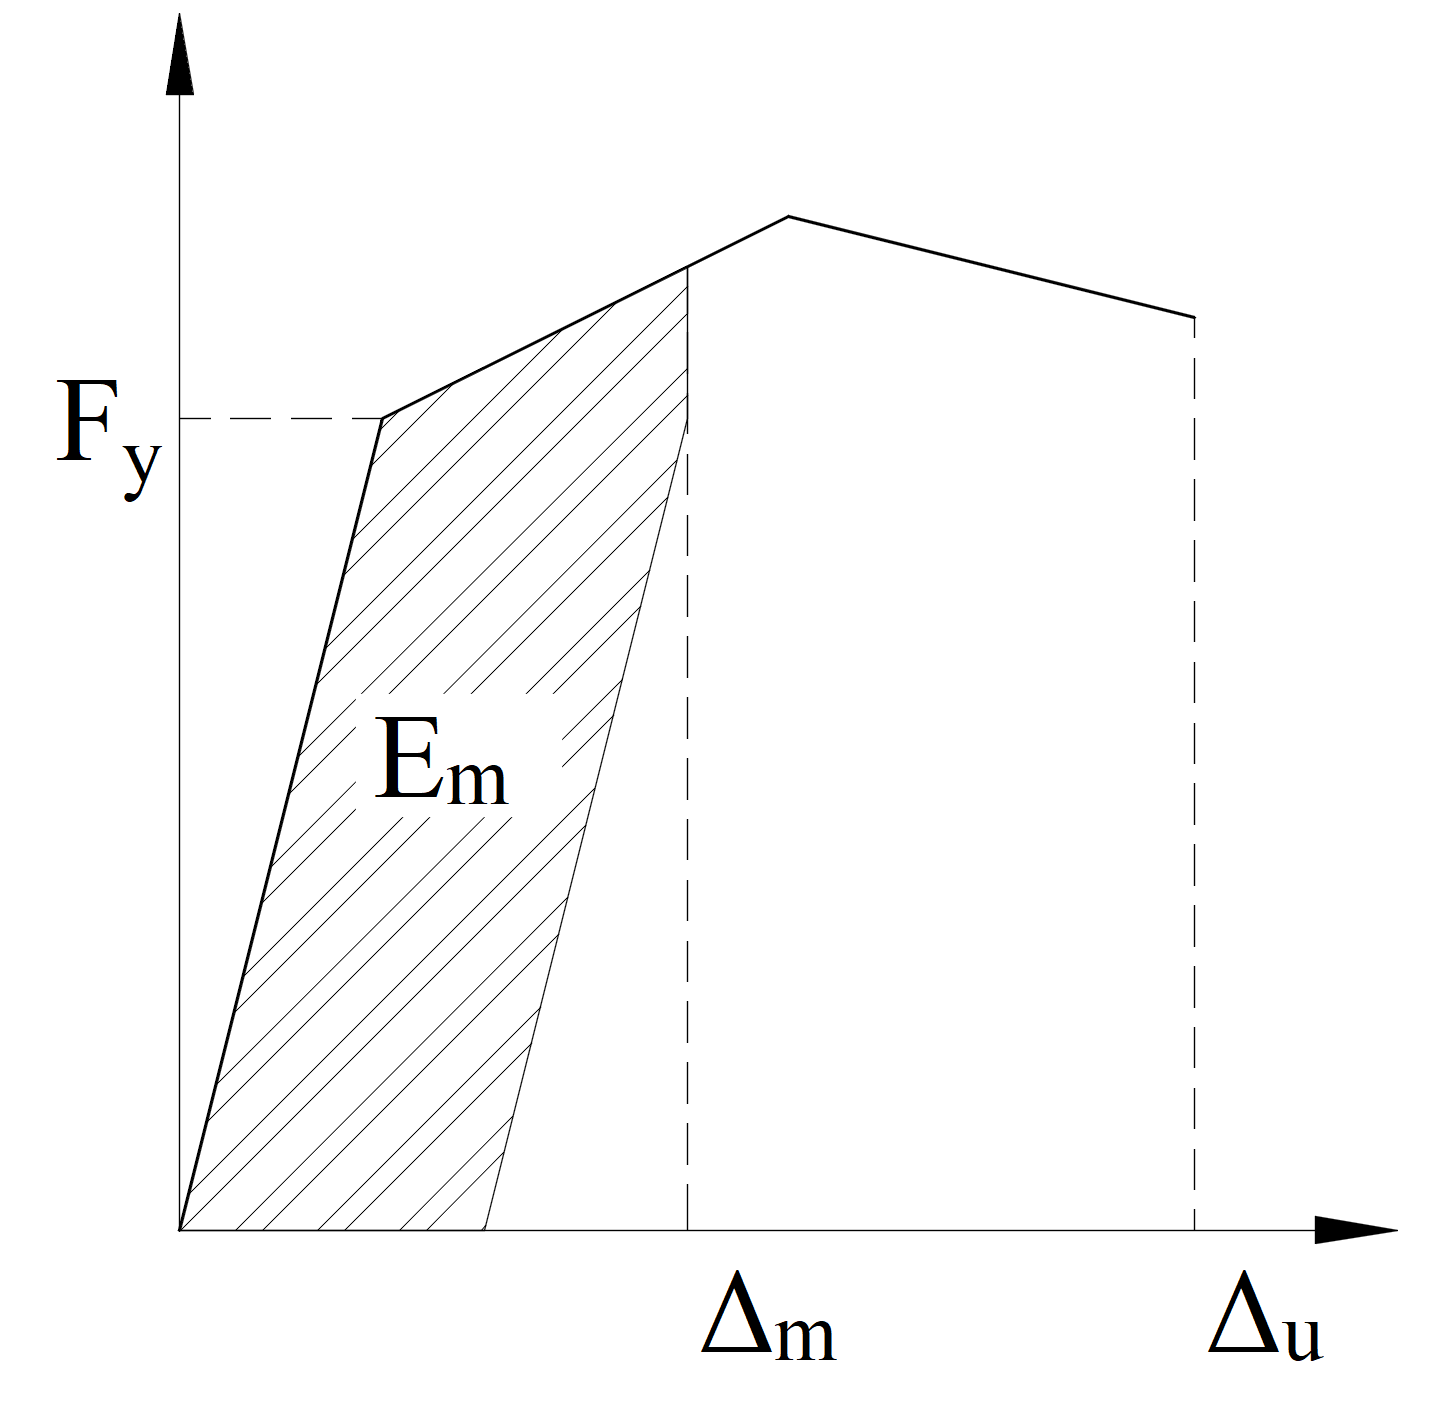
\includegraphics[width=0.6\textwidth]{Chapter-2/figs/Park_and_Ang_Model}
\caption{Park and Ang conceptual scheme}
\label{fig:Paa}
\end{figure}

Equation \ref{eq.DamageIndex} was derived for concrete elements. The first term here is a simple, pseudo-static displacement measure. The second term accounts for cumulative damage. A figure on the concept is shown in \fref{fig:Paa}. The advantages of this model are its simplicity and flexibility in adapting the model to correlate with experimental data.  

This model has several limitations. Firstly the calibration of the $\beta$ coefficient with observed damage has shown to be very low ($\beta=0.05-0.15$) \cite{Young-JiPark1985} \cite{Ghosh2015}, rendering the second term relatively inconsequential compared to the contribution of the first term. A sample result is taken from Gosh et al \cite{Ghosh2015}, which applied a modified version of the Park and Ang damage index in terms of the moment ($M_{y}$), the rotation ($\theta_y$), and curvature ductility ($\mu$) the modified model is expressed in equation \eref{eq.DamageIndexGhosh}.

\begin{equation}
	D=\frac{\mu_{m}}{\mu_{u}}-\beta\frac{E_h}{M_{y}\theta_y\mu{u}}
	\label{eq.DamageIndexGhosh}
\end{equation}

Using the following values: $\mu_{m}=4.93$; $\mu_{u}=17.02$; $M_{y}=8751.375$; $\theta_y=0.0042$; $E_{h}=119.07$; $\beta=0.05$ 

And substituting in equation \eref{eq.DamageIndexGhosh}:
\[
 D=\frac{\mu_{m}}{\mu_{u}}-\beta\frac{E_h}{M_{y}\theta_y\mu{u}}=0.3
	\]
\textbf{First term}:
\[
\frac{\mu_{m}}{\mu_{u}}=\frac{4.93}{17.02}=0.2897
\]
\textbf{Second term}: 
\[	
	\beta \frac{E_h}{M_{y}\theta_y\mu{u}}=0.05\frac{119.07}{8751.375*0.0042*17.02}=0.0103
\]

It can be seen that 97\% of the damage index comes from the first term which is the elastic term and the inelastic part is only 3\% of the total. 

Depite its limitation, several studies have used or modified this model to study the effects of cumulative damage for different structures,  of relevant importance are those performed by \cite{Kunnath1992}, who used a modified Park and Ang model, to model damagae at the local level for elements in a structural analysis program IDARC 3.0, in this software for the case of multiple degrees of freedom buildings they also added parameters to consider the damage at the inter-story level and the global model. Ghosh et al \cite{Ghosh2015} developed a damage accumulation framework to develop probabilistic estimates of exceeding a damage index for multiple ground motions. Other regressions have been proposed by \cite{Khashaee}, \cite{Fajfar1992}, \cite{Roufaiel} but show no improvement in assessing the damage state of a structure. While these studies provide an insight into some of the characteristics of damage accumulation they rely on the Park and Ang model and therefore carry the same limitations.

Krawinkler (1987) \cite{Krawinkler1987} proposed a method that considered damage as a function of low cycle fatigue parameters, the form of the Krawinkler damage index for steel components, weldments, and local buckling has a general shape of the Miner model. This model relies on the accumulation of plastic deformations. While this model has proven to work well for the evaluation of individual steel structure elements, it does not provide a way to generalize damage for other types of structures.


\section{Multiple earthquake loading}

The evaluation of multiple seismic events has been scarcely studied, however their effects have been felt in numerous earthquake sequences such as the Christchurch 2010, Umbria-Marche Earthquake 1997 and the Puerto Rico Earthquakes 2020. The hypothesis is that accumulation of damage will restart in a smaller seismic event to achieve a prescribed limit state, similar to how corrosion and other aging phenomena might impact the intensity needed to achieve a future limit state. 

In the literature the study of multiple earthquake loading can be classified in two groups:

\begin{itemize}
	\item Mainshock-aftershock sequences
	\item Mainshock sequences
\end{itemize}

These studies have shown what are some of the effects of multiple earthquake loading for different structures.

\subsection{Mainshock-aftershock sequences loading }

Strong aftershocks can increase the state of damage of a building or even collapse an already damaged structure. It is therefore important to quantify the increase of seismic demands in structures due to aftershock loading. In recent years different studies have been carried out to develop methodologies that consider these effects.

Tesfamariam et al \cite{Tesfamariam2015} investigated the increase in the demands for multiple degrees of freedom systems (MDOF). Their study carried out a parametric study RC frame buildings and RC frame with infill masonry buildings. A series of mainshock-aftershock sequences were applied. Their results showed that there is an increase of 10\% in the interstory drift demands for the RC frame structures. The authors did not check for strain limit states, therefore a damage limit state may have been reached, thus their study might have underestimated the structural performance. Simmilarly Raghunandan et al \cite{Raghunandan2015} studied the vulnerability of RC frame structure. Their study showed that depending on the level of interstory drift achieved during the mainshock the additional damage experienced during the aftershock will be different. For example, the authors showed that for an RC frame that experiences 4\% or more interstory drift in the mainshock, the median capacity to resist aftershock shaking is reduced by about 40\%. Furthermore, other studies have focused on the study of single degree of freedom (SDOF) systems response to mainshock-aftershock (MS-AS) sequences \cite{Hatzigeorgiou2009}\cite{Manafpour2019}. Hatzigeorgiou et al focused on determining the inelastic displacement coefficient variation due to the MS-AS sequence, their study concluded that there is an increase in the inelastic displacement demands, however, the limitations in their study did not reported what occurs to the performance limit states. Further, Manafpour et al studied the seismic drift behavior of structures to MS-AS sequences for far-field earthquakes and near-field earthquakes. Their study concluded that for SDOF structures near-field earthquake sequences were the most damaging, increasing the drifts by as much as 45\%.

Researchers have used two earthquake selection procedures. The first method incremental dynamic analysis (IDA) consists in 1)subject the nonlinear building model to a ground motion having a particular intensity, 2) record the response of the structure \cite{Vamvatsikos2002}, 3)in successive analyses, the ground motion is incrementally scaled to a higher intensity measure (IM), and 4)the structural response is recorded in each analysis. The IDA procedure was extrapolated to generate MS-AS sequence with to main steps: 1)Apply the IDA to the mainshocks to obtain different levels of damage in the structure, 2) after each mainshock include an incrementally scaled aftershock, and 3)Change the polarity of the aftershock, which refers to the direction of the aftershock variation to the mainshock. \fref{fig:MS-AS_Luco} shows one of the resulting MS-AS sequences using the IDA methodology. Due to the use of scaling factors the IDA methodology uses artificial mainshock-aftershock sequenceS. In addition, the IDA analysis can be computationally expensive, for example, the authors reported a total of 9900 ground motion sequences per structure.

\begin{figure}[htbp]
\centering
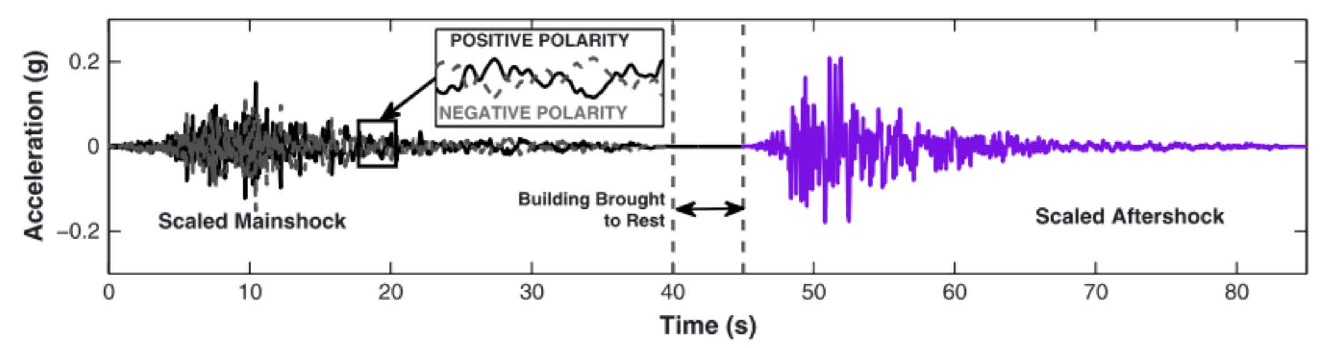
\includegraphics[width=0.6\textwidth]{Chapter-2/figs/MS-AS_sequence_Luco}
\caption{Mainshock-aftershock sequence train of ground motions \cite{Raghunandan2015}}
\label{fig:MS-AS_Luco}
\end{figure}

The second method consists in matching the MS-AS sequences to a site seismic hazard curve obtained from a probabilistic seismic hazard analysis (PSHA). Tesfamariam \cite{Tesfamariam2015} used conditional mean spectra (CMS) to match and select mainshock-aftershock sequences for structures located in Vancouver, BC. Their study selected MS-AS sequences from two databases of ground motions 1) NGA-West2 \citep{Ancheta2014}, and 2)K-NET//KiK-net \cite{NIEDK-NETKiK-net2019}. The CMS process consists in computing the expected response spectrum associated with a target spectral acceleration ($Sa$) value at a single period, using the known values from PSHA such as the magnitude, distance, and $\epsilon$ values. In their study the authors used CMS to select the MS-AS sequences for different earthquake scenarios a)Crustal earthquake, b) Interface, and c) Inslab, they hypothesized that different earthquake regimes would have different MS-AS sequence characteristics such as higher $Sa$ values at low periods for interface earthquakes or high values for crustal earthquakes. \fref{fig:MS-AS_Goda} shows this selection for a structure with a 0.4s period for crustal earthquakes. The CMS method adapts to the site conditions and no scaling of MS-AS is required since the selection is optimized to ground motion sequences stored in the databases. Since the CSM method uses site-specific data it can be a part of an analytical framework that can be adapted to different seismic regions.

\begin{figure}[htbp]
\centering
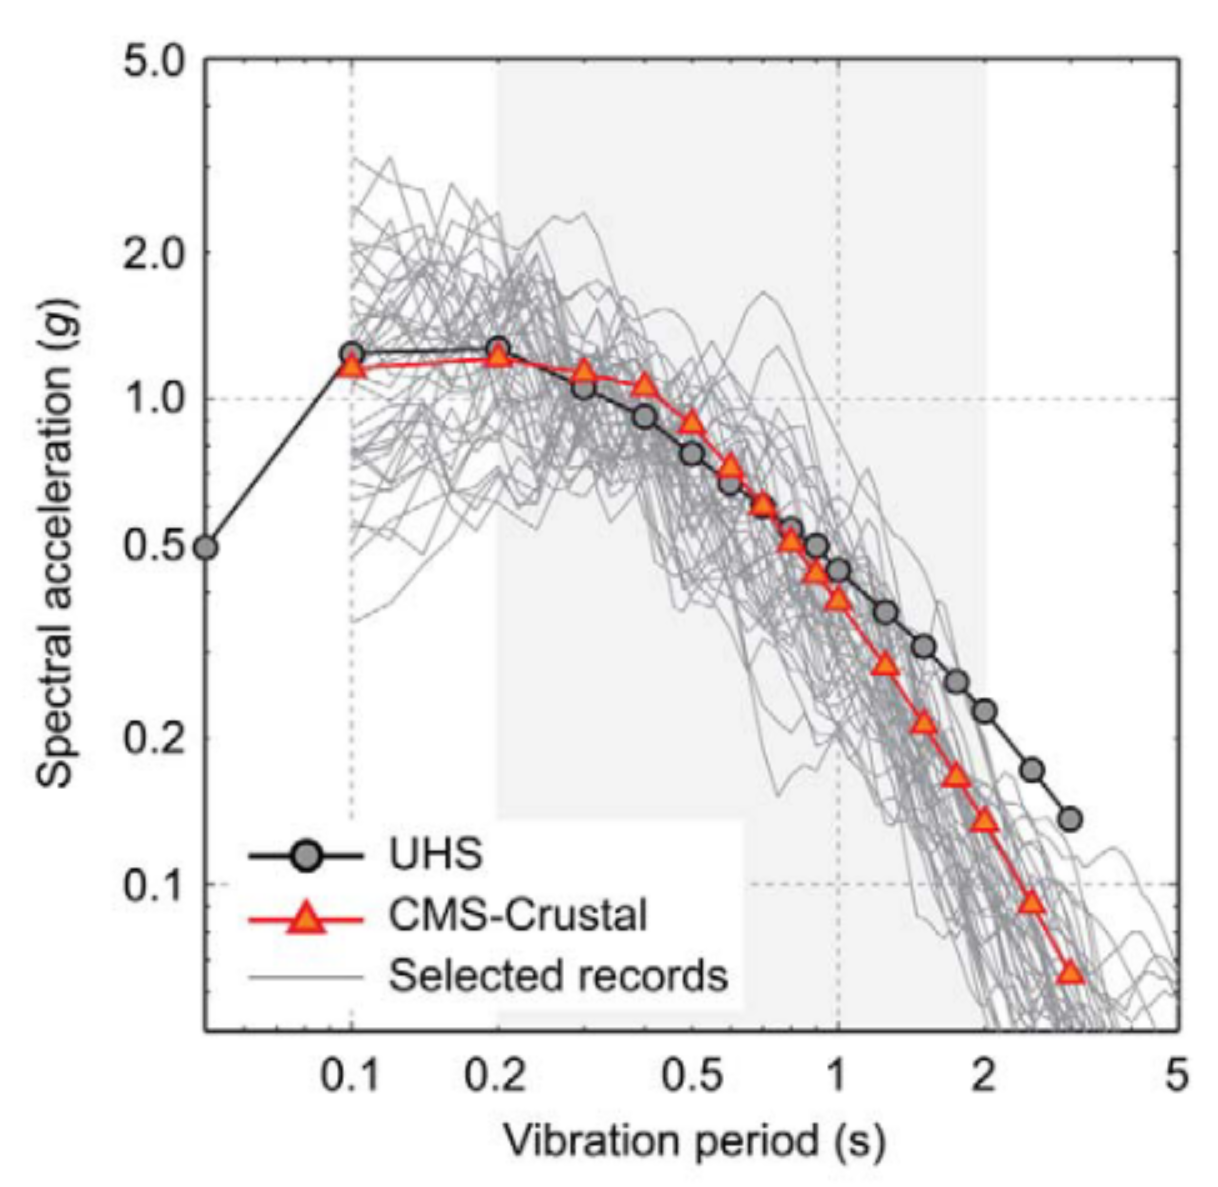
\includegraphics[width=0.5\textwidth]{Chapter-2/figs/CMS-Tesfamariam_MS-AS_seq}
\caption{Mainshock-aftershock sequence selection at T=0.4s for crustal earthquakes in Vancouver, British Coloumbia \cite{Tesfamariam2015}}
\label{fig:MS-AS_Goda}
\end{figure}

\subsection{Mainshock sequences loading}

Reliable prediction of earthquakes is currently impossible on any time scale.  However, for a large region, earthquakes recurence time can be modeled reasonably well as a Poisson process. Sunasaka \cite{Sunasaka1993} developed mainshock sequences that followed a Poisson process. Their study focused on the accumulation of damage due to mainshock sequences, and mainshocks-aftershocks sequences. Damage accumulation was accounted for by the Park and Ang index. The authors used ground motion prediction equations to develop artifficial mainshock sequences. Their study calculated the recurrence period, magnitude, location and peak ground acceleration for each of the mainshocks. The author subjected an SDOF bridge in Eureka, CA to the mainshock sequence shown in   \fref{fig:MS-MS_Sunasaka}. While the results shows a significant increase in the damage index due to mainshock sequences, the conclusion are limted by the assumption that a possion process can be applied to single faults which has not shown good correlation with observed events\cite{Shearer2009}. While this study shows what could be possible if mainshocks were predictable in small regions, more advances in seismology are needed to confidently apply the proposed methodology.

\begin{figure}[htbp]
\centering
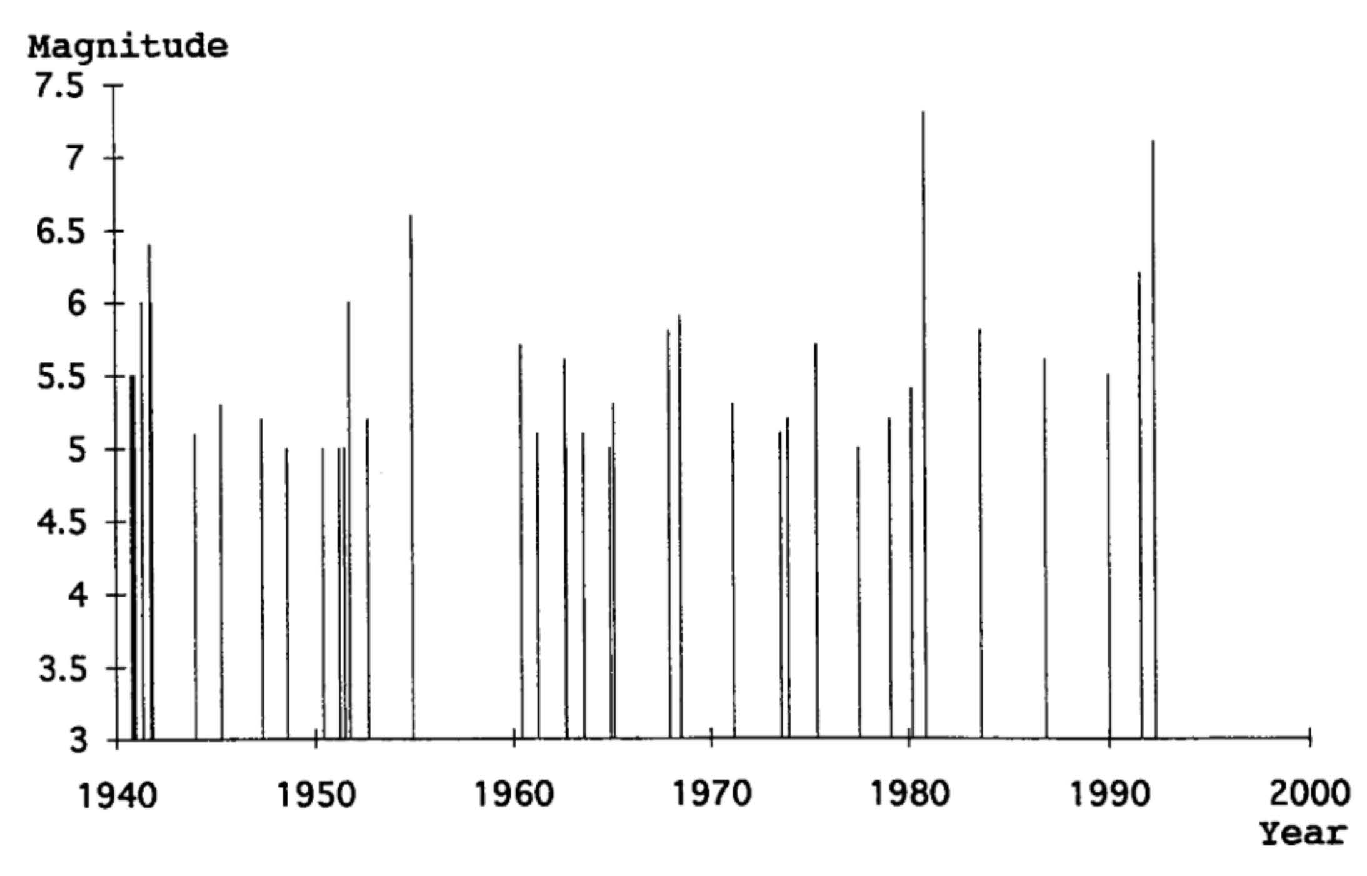
\includegraphics[width=0.5\textwidth]{Chapter-2/figs/Mainshock_sequence_01}
\caption{Mainshock sequence selection at Eureka, CA \cite{Sunasaka1993}}
\label{fig:MS-MS_Sunasaka}
\end{figure}

Other studies have used three equally spaced mainshocks \cite{Hatzigeorgiou2009}. The three equally spaced earthquake can be deployed without much computational effort, however, it as with the use of Poisson process methodology, there is not a seismological basis for the use of three equally spaced earthquakes. Therefore, the use of this methodology would be limited to scenario analysis and not very useful for design analysis.

\section{Aging of structures}

There have been attempts by many researchers to establish the best way to characterize the aging of structures.

In recent years studies have focused on the effect of cumulative damage. These studies have focused on assessing the damage accumulation under different loading conditions such as multiple earthquakes, corrosion and life span of the structure. Two main approaches to tackle this field of study have been observed:

\begin{itemize}
	\item Probabilistic framework
	\item Fragility curves
\end{itemize}

\textbf{Proababilistic Framework}

One of the most widely used probabilistic framework is the Pacific Earthquake Engineering Research Center (PEER) Performance Based Design. PEER PBD can be expressed by the following equation:
\begin{equation}
\nu_{DM}(dm^{LS})=\iint D_{DM|EDP}(dm|edp)|,dG_{EDP|IM}(edp|im)||\,d\nu_{IM}(im)|
\end{equation}

Mackie et al \cite{Mackie2007} on the basis of the PEER PBD developed the performance based damage design (PBDD) and performance based loss design (PBLD) by defining the probabilistic demand, damage, and loss model parameters in terms of reinforced concrete column damage. The RC column damage was defined in terms of drift ratios defined for the limit states of concrete spalling, bar buckling and failure. 

The authors show that for a given intensity measure (IM) and a confidence level of achieving a limit state, its is possible then to define the probability  of exceeding that limit state.

While this methodology was able to define damage and incorporate it into the PEER PBD framework, the authors did not consider  strain to define the limit states. Also recent research has shown that other intensity measures such as spectral displacement at effective first mode period ($S_{d}(T_{1})$) provide a better intensity measure \cite{Krish2018}.

\textbf{Fragility Curves}

Another common trend in this subject is the use of fragility curves to estimate the effect of damage in structures. Two main approaches were found in the literature. One of them relied on the Park and Ang Model damage index to define damage. While the second approach relates damage to drift.

Ghosh et al \cite{Ghosh2015} formulated a damage accumulation framework. Their study relied on the Park and Ang Damage index explained in the previous section. The study performed a series of nonlinear time history analyses for two cases:

\begin{itemize}
	\item Using a constant main shock hazard occurrence rate (3 main shocks in a 50 year period)
	\item Mainshock - Aftershock series using time-dependent aftershock hazard occurrence rate
\end{itemize}

Evaluation of the damage index exceeding probability for the two cases was performed. The results from this study show regression equations that statistically predict the damage index as a function of earthquake intensity and damage history. This study revealed that for both mainshock and aftershock scenarios there was a significant increase in the probability of damage index exceedance under repeated shock scenarios. While this study shows the importance of considering damage accumulation, these results have to be taken with caution since it carries the same disadvantages of the Park and Ang damage index.

Ghosh et al \cite{Ghosh2010} also studied the effects of corrosion in time dependent seismic fragility curves. Their study characterizes corrosion in concrete columns as a continuous phenomenon that occurs as a function of time. Additionally, the authors considered the effects of corrosion in steel bridge bearings. The authors then ran a series of NLTHA analyses for different aging times of the structures. Based on their analysis time dependent fragility curves were presented. The results showed that as time increases, and as a consequence corrosion increases, the probability of exceeding a limit state increases. In this study limit states where defined on the basis of inter-story drifts which were obtained from experimental results and field observations \cite{Padgett2007}. It is important to mention that the limit states used in their study, were not defined on the basis of strains or other structural property rather from a survey performed in central southeastern United States departments of transportation on the premise of a range of experienced inter-story drifts and the time to repair them. Additionally assuming that corrosion is a continuous process has to be cautiously taken as valid since site information such as temperature, water to cement ratio, the addition of cementitious materials such as silica fume, and the environment (e.g. coastal vs inland) affect the rate of propagation of corrosion\cite{Thoft-Christensen}.

While these studies provide a general view on how damage increases the likelihood of observing collapse or deterioration of the seismic performance, the methods used to arrive at those conclusions can be misleading since the definition of damage as either a Damage Index or Drift are not the best parameters to quantify the damage. It is our belief that strain-based limit states will provide a better understanding on the implications of damage accumulation.

\section{Research Gap}

It is clear that while studies have tried to show the importance of damage and multiple shocks through the lifetime of a structure, it is important to develop a model that establishes what is the likelihood of achieving a limit state as the structure ages. In addition,  it is important to understand the impacts of aging in bridge seismic performance. Furthermore, bridges in seismic areas can be subjected to main shock and aftershocks. Therefore a methodology that incorporates both aging and multiple events is needed.

Damage accumulation is topic that has been gaining momentum in the engineering community since these efforts will better inform  the potential future conditions of a structure to stakeholders such as state DOTs, building owners and practicing engineers, should the structure subjected to a further event. damage accumulation has been studied using the Park and Ang damage index or drift based limit states to measure damage accumulation. Different researchers have also included corrosion into their scope of analysis, which shows that aging conditions play an important role in the deterioration of a structure. In addition the literature uses the peak ground acceleration (PGA) as the controlling intensity measure (IM). This research will develop a parametric study using a series of single degree of freedom (SDOF) systems and subjecting them to different conditions such as corrosion, steel strain aging and strength aging among other. The SDOF structures will be subjected to a sweep of ground motions using nonlinear time history analysis to obtain maximum strain demands. With the results obtained fragility functions will be proposed for each limit state and aging condition. This research will provide the engineering community with a framework to account for damage in their analysis and guide decisions on the resiliency of a structure. In addition, this study will provide a methodology in which the Direct Displacement-Based Design (DDBD) is modified to consider the effects of damage and conditions.

\subsection{General Objectives}
The main goal of this research is to provide a methodology to consider damage into the PEER performance based design and demonstrate the implications of aging conditions and multiple earthquakes in the probability of collapse of a structure.

\subsection{Specific Objectives}
\begin{itemize}
	\item Incorporate different aging conditions and develop fragility curves that considers strain limit states as a measure of damage
	\item Establish limit states for corroded rebars
	\item Inform the research community on the necessary methodology to appropriately mimic real corrosion process in material experiments of corroded rebars, which can later be extrapolated to large scale testing of RC columns subjected to corrosion
	\item Consider the effects of multiple earthquakes for  two cases: (1) Mainshock sequences (2) Mainshock-Aftershock sequence
	\item Incorporate these results into the Direct Displacement Based Design (DDBD) methodology, through the use of factors that correspond to the aging conditions
\end{itemize}